
In this experiment we do not calibrate any pulse nor we characterize any qubit parameter, but rather we perform a practical evaluation of the quality of the calibration as well as a sanity check of the control system.

The experiment involves a set of gate defined as: $\{I,\,X,\,Y,\,X/2,\,Y/2\}$ where $I$ is the identity, $X-Y$ are \pipulse with relative phase of zero and $\pi/2$ respectively, and $X/2,\,Y/2$ are the same pulses with halved amplitude.
Talking in terms of rotation: we have $\pi$ and $\pi/2$ rotations along the X and Y axis, as well as two identity (correspondent to no pulse).

In an \textit{AllXY} experiment, we apply all the possible couples of gates of the defined set, one at a time, and perform a measurement.
In general, this experiment is referred in literature quoting not the probability of measuring the zero state nor the amplitude, but the expectation value of $\sigma_z$ ($1$ for $\ket 0$ and $-1$ for $\ket 1$).
So, we expect to measure $1$ for $\{II.\,XX,\,YY,\,XY,\,YX\}$, we expect $0$ for $\{IX/2,\,IY/2,\,XX/2,\,XY/2,\,X/2X,\,X/2Y,\\\,YX/2,\,YY/2,\,Y/2X,\,Y/2Y\}$ and finally $-1$ for $\{IX,\,IY,\,X/2X/2,\,Y/2Y/2\}$.

So, in the ideal case, a allXY plot looks like \cref{fig:sketch_allxy}.

\begin{figure}[ht]
    \centering
    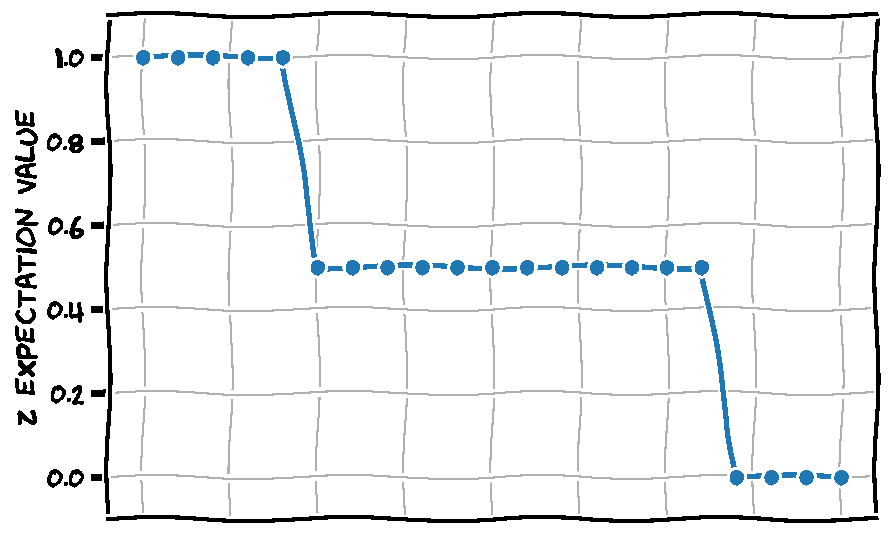
\includegraphics[width=0.5\textwidth]{characterization/figures/allxy_sketch.pdf}
    \caption{Ideal plot for a allXY experiment.}
    \label{fig:sketch_allxy}
\end{figure}

In a real case, usually, we have points more close to $0$ (the dephased state) as in \cref{fig:good_allxy}.
\begin{figure}[ht]
    \makebox[\textwidth][c]{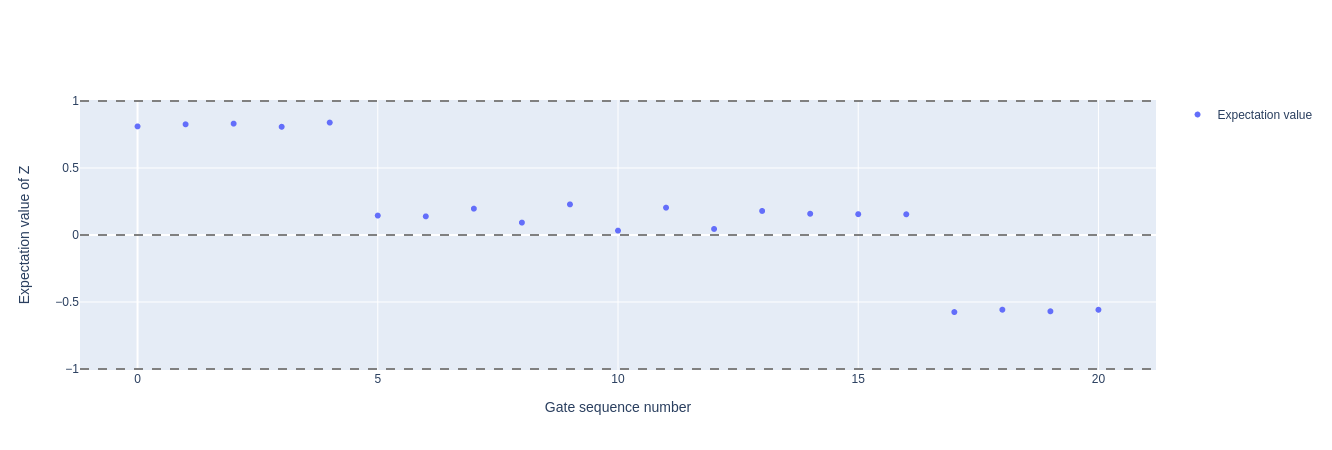
\includegraphics[width=1.3\textwidth]{characterization/figures/allxy.png}}
    \caption{Plot of a allXY experiment.}
    \label{fig:good_allxy}
\end{figure}

AllXY is extremely fast since it does not include any scan, but allows to see if the assignment fidelity is high enough and if the gate are working "together" properly in a single experiment.

Note also that, by looking at the kind of errors of allXY, we can infer which section of the calibration is most wrong~\cite{Gao2021}.

\experimentrecap
{AllXY}
{Healthcheck}
{None}
{select all the possible combination of couple of gates in the set composed of identity, \pipulse and \pihpulse with 0 and $\pi/2$ phase.
Execute a couple and measure, for all the couples.
Plot the expectation value of $\sigma_z$ for all the circuits performed and compare the results with the expect values}